\documentclass{article}

\usepackage[english]{babel}
\usepackage{tgtermes}
\usepackage{xcolor}
\usepackage{pagecolor}
\usepackage{hyperref}
\usepackage{graphicx}
\usepackage[labelformat=empty]{caption} 
\usepackage{amsfonts}
\usepackage{booktabs}
\usepackage{siunitx}
\usepackage{adjustbox}
\usepackage{caption}
\usepackage{float}


% % DRACULA COLORS
% \definecolor{draculabg}      {RGB} {25,   25,   25}
% \definecolor{draculacl}      {RGB} {68,   71,   90}
% \definecolor{draculafg}      {RGB} {248,  248,  242}
% \definecolor{draculacomment} {RGB} {98,   114,  164}
% \definecolor{draculacyan}    {RGB} {139,  233,  253}
% \definecolor{draculagreen}   {RGB} {80,   250,  123}
% \definecolor{draculaorange}  {RGB} {255,  184,  108}
% \definecolor{draculapink}    {RGB} {255,  121,  198}
% \definecolor{draculapurple}  {RGB} {189,  147,  249}
% \definecolor{draculared}     {RGB} {216,  47,   49}
% \definecolor{draculayellow}  {RGB} {241,  250,  140}
% \definecolor{draculablue}  {RGB} {36,  85,  151}


% DEFAULTS
\definecolor{draculabg}      {RGB} {255, 255, 255}
\definecolor{draculacl}      {RGB} {0,0,0}
\definecolor{draculafg}      {RGB} {0,0,0}
\definecolor{draculacomment} {RGB} {0,0,0}
\definecolor{draculacyan}    {RGB} {0,0,0}
\definecolor{draculagreen}   {RGB} {0,0,0}
\definecolor{draculaorange}  {RGB} {0,0,0}
\definecolor{draculapink}    {RGB} {0,0,0}
\definecolor{draculapurple}  {RGB} {0,0,0}
\definecolor{draculared}     {RGB} {0,0,0}
\definecolor{draculayellow}  {RGB} {0,0,0}
\definecolor{draculablue}  {RGB} {0,0,0}

\pagecolor{draculabg}
\color{draculafg}

\nocite{*}

\title{\textbf{Aldone}}
\author{Fausto Zamparelli, Daniel Falbo}
\date{May 30, 2024}

\hypersetup{
colorlinks=true,
linkcolor=draculapurple,
citecolor=draculapurple,
urlcolor=draculapurple,
pdftitle={Aldone},
pdfpagemode=FullScreen,
}

\begin{document}

\maketitle

\section*{\color{draculagreen}Introduction}
Aldone as in "AI-Done" is a tool for personal reminders and grocery list management.
This is a proof of concept of a product that could save you time every day by allowing you
to smoothly interact with it on the fly.

Aldone is a react web app that interacts with a node.js and a python server doing most of the magic.
After a log-in you will be able to speak to it to add tasks to your grocery list, to-do list,
or make questions about reminders you saved earlier.
Furthermore, you could ask to split a task in sub-tasks or approximate how long a task will take.
Aldone is able to detect fully by himself weather you are asking him to add something to your grocery list or to-do list.

The coolest thing is that once you will come home from the supermarket with tired legs and arms from carrying bags, you won't have to manually remove everything from this digital grocery list but you can use your phone camera to detect what foods you actually bought and then Aldone will remove them for you. Other use cases for this include checking what's already in your kitchen or marking products as bought after delegating your groceries to someone else.

\newpage

\section*{\color{draculagreen}Method} 
\begin{figure}[htbp]
\centering
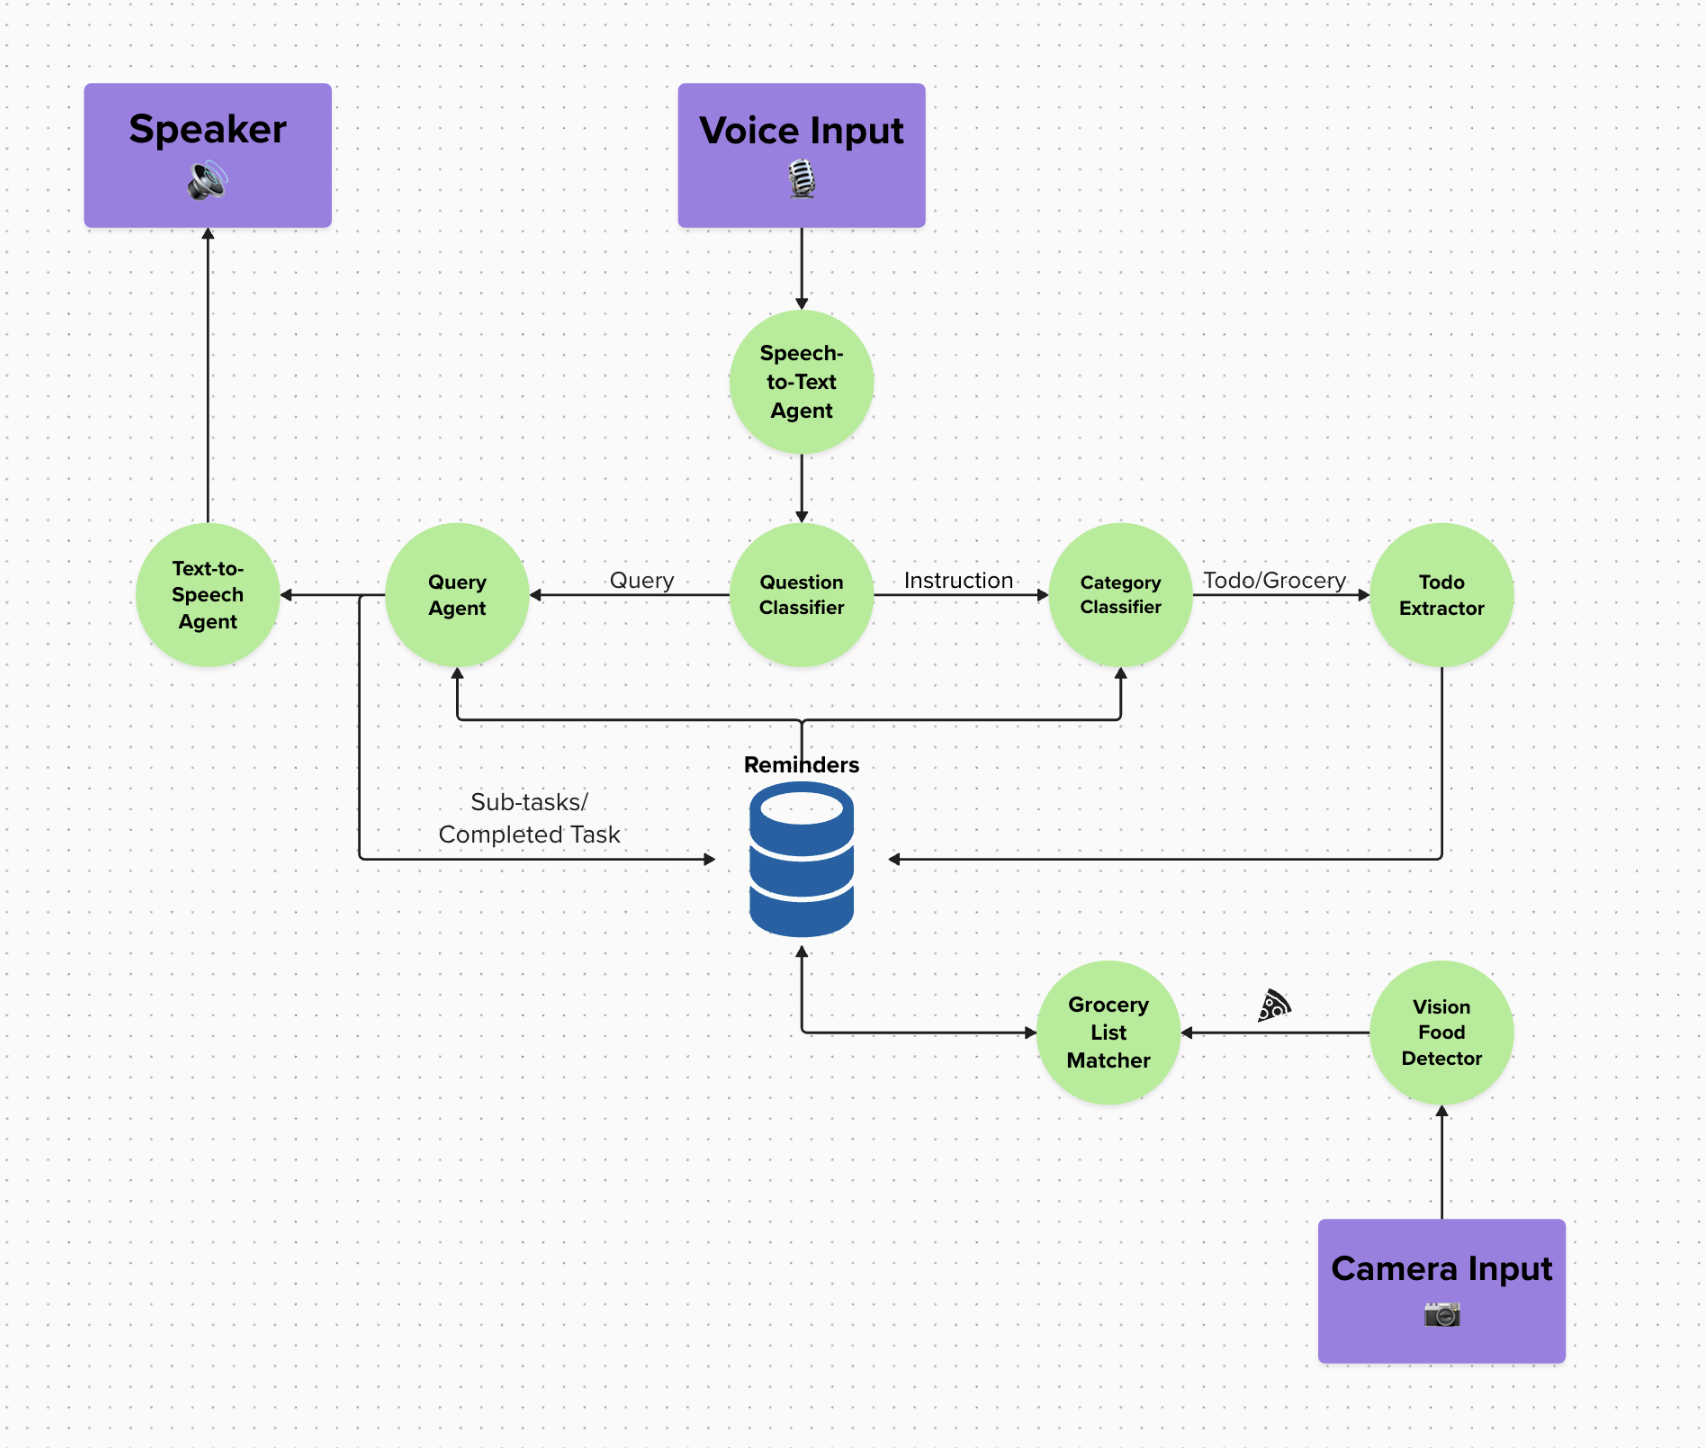
\includegraphics[width=\textwidth]{diagram.png}
\caption{\small Visual representation of the agents that make up Aldone}
\end{figure}

As we can see Aldone was created by splitting its behind-the-scenes functionalities into multiple specialized AI agents that cooperate with each others. In order to fully understand how Aldone works under the hood it is best to understand the functionality of each of these agents alone. Let's work our way thorough the graph from top to bottom:

\subsection*{\color{draculayellow}Speech-to-Text Agent}
For the Speech-to-Text task, being a web app, Aldone uses the browser's built-in Web Speech API service for convenience. The implementation can be found by searching for ``webkitSpeechRecognition" in the `src/app/[username]/page.tsx' file.

\newpage

\subsection*{\color{draculayellow}Question Classifier}
The task of the Question Classifier is to determine whether the user's input is a question/query or a statement/instruction. Anything that involves looking for information in the web or from the existing data in the database, is a query. Anything that provides new data within the input, is not a query.

\begin{figure}[H]
\begin{center}
\begin{tabular}{SS}
  \toprule
    \text{Input} & \text{Label} \\
    \midrule
    \text{``What's the capital of Italy?"}  & \text{Query} \\
    \text{``Add milk to my grocery list"}  & \text{Not Query}  \\
    \text{``Split task X into subtasks"} & \text{Query}  \\
    \bottomrule
\end{tabular}
\end{center}
\caption{\it For example, the input "What's the capital of Italy?" is a query, while "Add milk to my grocery list" is an instruction. The input "Split task X into subtasks" is also a query because the data is not being provided by the input.} \label{faketable:mul}
\end{figure}


The Question Classifier is implemented using a neural network trained on a dataset of 500 examples.
The question classifier is a pytorch neural network and its code can be found in the subdirectory ``src/py/question\_classifier''.

In the subdirectory,
\begin{itemize}
 \item \texttt{nndata.json}: is the dataset used to train the model
  \item \texttt{nntraining.py}: is the training script that generates the model. 80\% of the data is used for training and 20\% for testing. Of the training data, 25\% is used for validation.
  \item \texttt{nnlabeler.py}: uses the trained model to label new input data.
\end{itemize}

\begin{figure}[htbp]
\centering
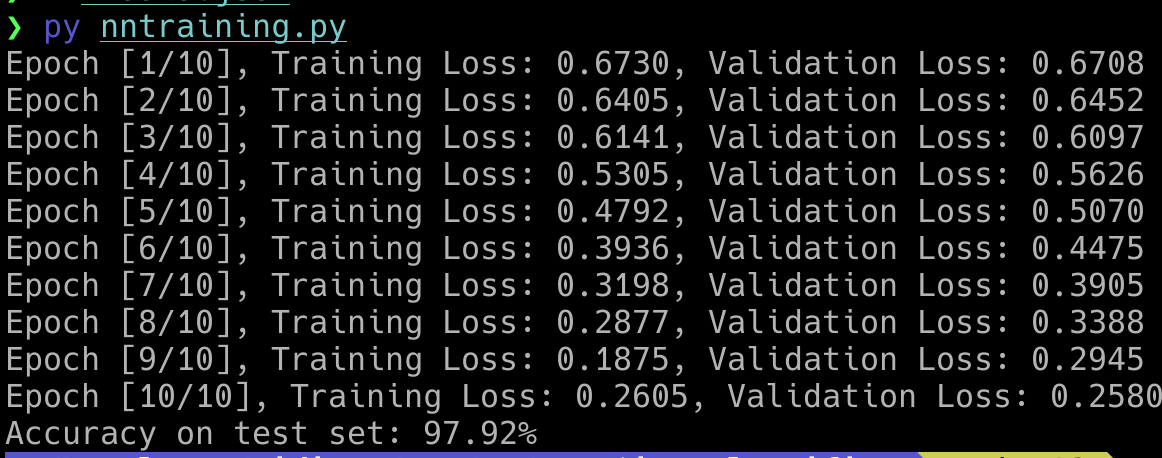
\includegraphics[width=\textwidth]{question_classifier_accuracy.png}
\caption{\small We achieved 97\% accuracy on the test set. Of course it's still a small dataset and more data would make it more solid.}
\end{figure}

\subsection*{\color{draculayellow}Category Classifier}

\subsection*{\color{draculayellow}Todo Extractor}

[Confusion Matrix here]

\subsection*{\color{draculayellow}Vision Food Detector}

We first asked the LLM model to give us the entire updated grocery list object, but empirically it often made errors. What we ended up doing is asking the LLM model for indices of the grocery list that were updated, and then we updated the grocery list object ourselves. This way, we could ensure that the grocery list object was updated correctly.

\subsection*{\color{draculayellow}Grocery List Matcher}

\subsection*{\color{draculayellow}General Agent}

\subsection*{\color{draculayellow}Text-to-Speech Agent}

\section*{\color{draculagreen}Results}

\subsection*{\color{draculagreen}Glue Orchestration}

\section*{\color{draculagreen}Source of inspiration}

[1] \href{https://humane.com/media/cosmos-an-operating-system-for-the-ai-era}{Cosmos: An Operating System for the AI Era} \newline
[2] aiXplain

\end{document}
